\input templates/header
\title[ASD - Approssimazione]{\textbf{Algoritmi e Strutture Dati}\\[24pt]Tecniche risolutive per problemi intrattabili}

\usepackage{epigraph}
\usepackage{xcolor}
\usepackage{colortbl}

\newcommand{\PTIME}{\mbox{\sc $\mathbb{P}$}}
\renewcommand{\NP}{\mbox{$\mathbb{NP}$}}
\newcommand{\TIME}{\mbox{$\mathbb{TIME}$}}
\newcommand{\EXPTIME}{\mbox{$\mathbb{EXPTIME}$}}
\newcommand{\SPACE}{\mbox{$\mathbb{SPACE}$}}
\newcommand{\PSPACE}{\mbox{$\mathbb{PSPACE}$}}

\newcommand{\R}[1]{\textcolor{red}{#1}}
\newcommand{\B}[1]{\textcolor{blue}{#1}}

\renewcommand{\arraystretch}{1.4}
\graphicspath{{figs/19/}}
\renewcommand{\enumerazione}{\fontproc{enumeration}}
\newcommand{\isAdmissible}{\fontproc{isAdmissible}}

\begin{document}

%-------------------------------------------------------------------------
\FrameTitle{}

%-------------------------------------------------------------------------
\begin{PlainFrame}{Sommario}
\TwoCols{
  \tableofcontents
}{
 \epigraph{Chi si accontenta, gode}{Proverbio}

 \bigskip
 \epigraph{Le mieux est l’ennemi du bien\\Il meglio è nemico del bene}{Voltaire, La Bégueule, 1772}
  
}
\end{PlainFrame}



%%%%%%%%%%%%%%%%%%%%%%%%%%%%%%%%%%%%%%%%%%%%%%%%%%%%%%%%%%%%%%%%%%%%%%%%%%
\section{Introduzione}


%-------------------------------------------------------------------------
\begin{frame}{Introduzione}


Non si può avere tutto dalla vita; bisogna rinunciare a qualcosa:
\BIL
\item \B{Generalità}: 
  \BI
  \item Algoritmi \alert{pseudo-polinomiali} che funzionano per
    solo alcuni casi particolari dell'input
  \EI
\item \B{Ottimalità}: 
  \BI
  \item Algoritmi di \alert{approssimazione}, che garantiscono di ottenere soluzioni "vicine" alla soluzione ottimale
  \EI
\item \B{Efficienza}:
  \BI
  \item Algoritmi esponenziali \alert{branch-\&-bound}, che limitano lo spazio di ricerca con un'accurata potatura
  \EI
\item \B{Formalità}: 
  \BI
  \item Algoritmi \alert{euristici}, di solito basati su tecniche greedy o di ricerca locale, che forniscano sperimentalmente risultati buoni
  \EI
\EIL

\end{frame}

\section{Algoritmi pseudo-polinomiali}

%-------------------------------------------------------------------------
\begin{frame}{Subset-Sum}

\vspace{-9pt}
\begin{myboxtitle}[Somma di sottoinsieme (Subset sum)]
Dati un insieme $A = \{ a_1 , \mldots, a_n\}$ di interi positivi ed un intero
positivo $k$, esiste un sottoinsieme $S$ di indici in $\{1, \mldots, n\}$ tale
che $\sum_{i \in S} a_i = k$?
\end{myboxtitle}

\IG{0.60}{subsetsum.png}

\vfill
\tiny
\url{https://xkcd.com/287/}

\end{frame}

%-------------------------------------------------------------------------
\begin{frame}{Subset Sum}

Definiamo una tabella booleana $DP[0 \ldots n][0 \ldots k]$. 

$DP[i][r]$ è uguale a \TRUE se e solo se esiste un sottoinsieme dei primi $i$ valori memorizzati in $A$ la cui somma è pari a $r$.

\[
DP[i][r] = \begin{cases}
  \FALSE & r < 0 \\
  \TRUE & r = 0 \\
  \FALSE & r > 0 \wedge i=0 \\
  DP[i-1][r]\ \OR\ DP[i-1][r-A[i]] & r>0 \wedge i>0
\end{cases}
\]

\bigskip
Essendo un problema decisionale:
\BIL 
\item è possibile semplificare e utilizzare spazio $\Theta(k)$ invece che $\Theta(nk)$
\item la complessità resta $\Theta(nk)$
\EIL

\end{frame}

%-------------------------------------------------------------------------
\begin{frame}{Subset Sum}

\begin{Procedure}
\caption[A]{\BOOLEAN \subsetsum($\INTARRAY\ A,\ \INTEGER\ n,\ \INTEGER\ k$)}

$\BOOLEAN[\,]\ DP = \NEW\ \BOOLEAN[0 \mldots n][0 \mldots k]$\;
$DP[0][0] = \TRUE$\;
\For{$r = 1$ \TO $k$}{
  $DP[0][r] = \FALSE$\;
}
\For{$i = 1$ \TO $n$}{
  \For{$r = A[i]$ \TO $k$}{
    $DP[i][r] = DP[i-1][r]\ \OR\ DP[i-1][r-A[i]]$\;
  }
}
\Return $DP[n][k]$\;
\end{Procedure}

\end{frame}

%-------------------------------------------------------------------------
\begin{frame}{Subset Sum}

Input: $A = [7, 11, 13], k=24$

\bigskip
\IG{1.0}{table.pdf}

\end{frame}

%-------------------------------------------------------------------------
\begin{frame}{Complessità}

\vspace{-9pt}
\begin{myboxtitle}[Analisi complessità]
\BIL
\item Complessità: $O(nk)$
\item Dimensione dei dati in ingresso: $O(n \log k)$, in quanto $\forall i: A[i] \leq k$ (valori più grandi possono essere esclusi)
\item Se $k = O(n^c)$ con $c$ costante, allora $\subsetsum$ ha complessità
polinomiale $O(n^{c+1})$
\item Se $k = O(2^n)$, allora $\subsetsum$ ha complessità superpolinomiale
$O(n2^n)$
\EIL
\end{myboxtitle}

\begin{myboxtitle}[Osservazione]
La complessità di \subsetsum() non dipende soltanto dalla 
cardinalità $n$ dell'insieme in ingresso, ma anche dai valori contenuti
nell'insieme
\end{myboxtitle}

\end{frame}

%-------------------------------------------------------------------------
\begin{frame}{Problemi fortemente \NP-completi}

\vspace{-9pt}
\begin{myboxtitle}[Dimensioni del problema]
Dato un problema decisionale $R$ e una sua istanza $I$:
\BIL
\item La \alert{dimensione $d$} di $I$ è la lunghezza della stringa che codifica $I$
\item Il \alert{valore \#} è il più grande numero intero che appare in $I$
\EIL
\end{myboxtitle}

\bigskip
\BB{Esempi}
\medskip
\small
\begin{tabular}{|c|c|c|c|}
\hline
\textbf{Nome} & $I$ & \# & $d$ \\\hline
\textsc{subset-sum} & $ \{n, k, a_1, \ldots, a_n\}$ & $\max\{n, k, \max \{ a_i \}\}$ & $O(n \log \#)$ \\\hline
\textsc{tsp} & $\{n, k, [d_{ij}]\}$ & $\max\{n, k, \max \{ d_{ij} \}\}$ &
$O(n^2 \log \#)$ \\\hline
\textsc{clique} & $\{n, m, k, G \}$ & $\max\{n, m, k\}$ & $O(n + m+ \log\#)$\\\hline
\end{tabular}

\end{frame}

%-------------------------------------------------------------------------
\begin{frame}{Problemi fortemente \NP-completi}

\vspace{-9pt}
\begin{myboxtitle}[Definizione]
Sia $R_p$ il problema $R$ ristretto a quei dati d'ingresso per i quali \# è
limitato superiormente da $p(d)$, con $p$ funzione polinomiale in $d$. $R$ è
\alert{fortemente \NP-completo} se $R_p$ è \NP-completo
\end{myboxtitle}

\begin{myboxtitle}[Esempio -- \textsc{clique} è fortemente \NP-completo]
\BIL
\item $k \leq n$ (altrimenti la risposta è \FALSE)
\item $\# = \max \{ n, m, k \} = \max \{ n, m \}$
\item $d = O(n + m + \log \#) = O(n+m)$
\item Quindi $\# = \max \{ n, m \}$ è limitato superiormente da $O(n+m)$
\item Il problema ristretto è identico a \textsc{clique}, che è \NP-completo
\EIL
\end{myboxtitle}

\end{frame}

%-------------------------------------------------------------------------
\begin{frame}{Problemi debolmente \NP-completi}

\vspace{-9pt}
\begin{myboxtitle}[Definizione]
Se un problema \NP-completo non è fortemente \NP-completo, allora è \alert{debolmente \NP-completo}.    
\end{myboxtitle}

\begin{myboxtitle}[Esempio -- \textsc{subset-sum} è debolmente \NP-completo]
\BIL
\item $\forall a_i \leq k$ (valori più grandi di $k$ vanno esclusi)
\item Se $k=O(n^c)$, allora $\# = \max \{n, k, a_1, \ldots, a_n\} = O(n^c)$
\item La soluzione basata su programmazione dinamica ha complessità
$O(nk) = O(n^{c+1})$, quindi in $\PTIME$.
\item Quindi \textsc{subset-sum} non è fortemente \NP-completo
\EIL
\end{myboxtitle}

\end{frame}

%-------------------------------------------------------------------------
\begin{frame}{Algoritmi pseudo-polinomiale}

\vspace{-9pt}
\begin{myboxtitle}[Definizione]
Un algoritmo che risolve un certo problema $R$, per qualsiasi
dato $I$ d'ingresso, in tempo $p(\#, d)$, con $p$ funzione polinomiale in $\#$
e $d$, ha complessità \alert{pseudo-polinomiale}.
\end{myboxtitle}

\begin{myboxtitle}[Esempio]
L'algoritmo che abbiamo visto per \textsc{subset-sum} è pseudo-polinomiale
\end{myboxtitle}

\begin{myboxtitle}[Teorema]
Nessun problema fortemente \NP-completo può essere risolto da un algoritmo
pseudo-polinomiale, a meno che non sia $\PP = \NP$.
\end{myboxtitle}

\end{frame}

%-------------------------------------------------------------------------
\begin{frame}{Problemi debolmente/fortemente \NP-completi}

\vspace{-9pt}
\begin{myboxtitle}[Partizione (\textsc{partition})]
Dato un insieme $A = \{ a_1, \mldots, a_n\}$ di interi positivi, esiste un
sottoinsieme $S$ di \{1, \mldots, n\} tale che $\sum_{i\in S} a_i = \sum_{i
\notin S}a_i$?
\end{myboxtitle}

\begin{myboxtitle}[Esempio]
\begin{overprint}
\onslide<1|handout:0>
\begin{tabular}{|c|c|c|c|c|c|}
\hline
14 & 6 & 12 & 3 & 7 & 2 \\\hline
\end{tabular}
\onslide<2|handout:1>
\begin{tabular}{|c|c|c|c|c|c|}
\hline
\R{14} & \R{6} & \B{12} & \B{3} & \B{7} & \R{2} \\\hline
\end{tabular}
\end{overprint}
\end{myboxtitle}

\begin{myboxtitle}[Domanda -- \textsc{partition} è debolmente \NP-completo?]

\pause
Sì, perchè è possibile ridurlo a \textsc{subset-sum} scegliendo come
valore $k$ la metà di tutti i valori presenti:

\[
  k = \frac{\sum_{i=1}^n a_i}{2} = \frac{44}{2} = 22
\]
\end{myboxtitle}

\end{frame}



%-------------------------------------------------------------------------
\begin{frame}{Problemi debolmente/fortemente \NP-completi}

\vspace{-9pt}
\begin{myboxtitle}[3-Partizione (\textsc{3-partition})]
Dati $3n$ interi $\{a_1, \mldots, a_{3n}\}$, esiste una partizione in $n$
triple $T_1, \mldots, T_n$, tale che la somma dei tre elementi di ogni $T_j$ è
la stessa, per $1 \le j \le n$?
\end{myboxtitle}

\begin{myboxtitle}[Domanda -- \textsc{3-partition} è debolmente \NP-completo?]
\pause
No, non esiste un algoritmo psuedo-polinomiale per risolvere 3-partition.
\end{myboxtitle}

\end{frame}

%%%%%%%%%%%%%%%%%%%%%%%%%%%%%%%%%%%%%%%%%%%%%%%%%%%%%%%%%%%%%%%%%%%%%%%%%%
\section{Algoritmi di approssimazione}

%-------------------------------------------------------------------------
\begin{frame}{Algoritmi di approssimizzazione}

\vspace{-9pt}
\begin{myboxtitle}[Premessa]
\BIL
\item I problemi più interessanti sono in forma di ottimizzazione
\item Tali problemi sono "più difficili" dei corrispondenti problemi
in forma di decisione
\item Se il problema di decisione è \NP-completo, non sono noti 
algoritmi polinomiali per il problema di ottimizzazione
\item Esistono algoritmi polinomiali che trovano soluzioni ammissibili
più o meno vicine a quella ottima
\EIL
\end{myboxtitle}

\begin{myboxtitle}[Algoritmi di approssimazione]
Se è possibile dimostrare un limite superiore/inferiore al rapporto fra la soluzione trovata e la soluzione ottima, allora tali algoritmi
vengono detti \alert{algoritmi di approssimazione}.
\end{myboxtitle}

\end{frame}

%-------------------------------------------------------------------------
\begin{frame}{Approssimazione}

\vspace{-9pt}
\begin{myboxtitle}[Definizione]
Dato un problema di ottimizzazione con funzione costo non negativa $c$,
un algoritmo si dice di \alert{$\alpha(n)$-approssimazione} se fornisce una soluzione ammissibile $x$ il cui costo $c(x)$ non si discosta dal costo $c(x^*)$ della soluzione ottima $x^*$ per più di un fattore $\alpha(n)$,
per qualunque input di dimensione $n$:

\begin{align*}
c(x^*) \leq c(x) & \leq \alpha(n) c(x^*)  && \alpha(n) > 1 \qquad (\textrm{Minimizzazione})\\
\alpha(n) c(x^*) \leq c(x) & \leq c(x^*)  && \alpha(n) < 1 \qquad (\textrm{Massimizzazione})
\end{align*}
\end{myboxtitle}

\BIL
\item $\alpha(n)$ può essere una costante, valida per tutti gli $n$
\item Identificare un valore $\alpha(n)$ e dimostrare che l'algoritmo lo rispetta è ciò che rende un buon algoritmo un algoritmo di approssimazione
\EIL


\end{frame}


%-------------------------------------------------------------------------
\begin{frame}{Esempio}

\vspace{-9pt}
\begin{myboxtitle}[Bin packing]
Dati:
\BI
\item un vettore $A = [a_1, \mldots, a_n]$ di interi positivi (i \alert{volumi}
di $n$ \alert{oggetti}) 
\item un intero positivo $k$ (la \alert{capacità} di una \alert{scatola}, tale che $\forall i: a_i \leq k$), 
\EI
si vuole trovare una partizione di $\{1, \mldots, n\}$ nel minimo numero di sottoinsiemi disgiunti (``scatole'') tali che $\sum_{i\in S} a_i \le k$ per ogni insieme $S$ della partizione
\end{myboxtitle}

\vspace{-9pt}
\TwoColsCustom{0.45}{0.53}{
\begin{myboxtitle}[Esempio]
\begin{tabular}{|c|c|c|c|c|c|c|}
\hline
3 & 7 & 2 & 5 & 4 & 3 & 5 \\\hline
\end{tabular}
\end{myboxtitle}
}{
\begin{myboxtitle}[Domanda]
Come risolvereste il problema?
\end{myboxtitle}
}

\end{frame}

%-------------------------------------------------------------------------
\begin{frame}{First-fit}

\vspace{-9pt}
\begin{myboxtitle}[Algoritmo \textsc{first-fit}]
Gli oggetti sono considerati in un ordine qualsiasi e ciascun oggetto è assegnato alla prima scatola che lo può contenere, tenuto conto di quanto
spazio è stato occupato della stessa. (Algoritmo Greedy)
\end{myboxtitle}

\bigskip
\BB{Esempio}

\bigskip
\begin{tabular}{|c|c|c|c|c|c|c|}
\hline
3 & 7 & 2 & 5 & 4 & 3 & 5 \\\hline
\end{tabular}

\bigskip
$k=8$

\bigskip
\begin{overprint}

\onslide<1|handout:0>
\begin{tabular}{|P{1.1cm}|P{1.1cm}|P{1.1cm}|P{1.1cm}|P{1.1cm}|}
\hline
&&&& \\\hline
\end{tabular}

\onslide<2|handout:0>
\begin{tabular}{|P{1.1cm}|P{1.1cm}|P{1.1cm}|P{1.1cm}|P{1.1cm}|}
\hline
3 &&&& \\\hline
\end{tabular}

\onslide<3|handout:0>
\begin{tabular}{|P{1.1cm}|P{1.1cm}|P{1.1cm}|P{1.1cm}|P{1.1cm}|}
\hline
3 & 7 &&& \\\hline
\end{tabular}

\onslide<4|handout:0>
\begin{tabular}{|P{1.1cm}|P{1.1cm}|P{1.1cm}|P{1.1cm}|P{1.1cm}|}
\hline
3, 2 & 7 &&& \\\hline
\end{tabular}

\onslide<5|handout:0>
\begin{tabular}{|P{1.1cm}|P{1.1cm}|P{1.1cm}|P{1.1cm}|P{1.1cm}|}
\hline
3, 2 & 7 & 5 && \\\hline
\end{tabular}

\onslide<6|handout:0>
\begin{tabular}{|P{1.1cm}|P{1.1cm}|P{1.1cm}|P{1.1cm}|P{1.1cm}|}
\hline
3, 2 & 7 & 5 & 4 & \\\hline
\end{tabular}

\onslide<7|handout:0>
\begin{tabular}{|P{1.1cm}|P{1.1cm}|P{1.1cm}|P{1.1cm}|P{1.1cm}|}
\hline
3, 2, 3 & 7 & 5 & 4 &\\\hline
\end{tabular}

\onslide<8|handout:1>
\begin{tabular}{|P{1.1cm}|P{1.1cm}|P{1.1cm}|P{1.1cm}|P{1.1cm}|}
\hline
3, 2, 3 & 7 & 5 & 4 & 5 \\\hline
\end{tabular}

\end{overprint}

\end{frame}

\begin{frame}{Approssimazione First-Fit}

\vspace{-12pt}
\BIL
\item Sia $N>1$ il numero di scatole usate da \textsc{first-fit}\\ 
(se $N=1$, \textsc{first-fit} è ottimale)

\item Il numero minimo di scatole $N^*$ è limitato da:
\medskip
\[
  N^* \geq \frac{\sum_{i = 1}^{n} a_i}{k} = \frac{29}{8}  =  3.625
\]
\item Non possono esserci due scatole riempite meno della metà:
\medskip
\[
  N < \frac{\sum_{i = 1}^{n} a_i}{k/2} = \frac{29}{8/2} = 7.250 
\]

\item Abbiamo quindi:
\[
 N < \frac{\sum_{i = 1}^{n} a_i}{k/2} = 2 \frac{\sum_{i = 1}^{n} a_i}{k/2} \leq 2 N^* = \alpha(n) N^*
\]
che implica $\alpha(n) = 2$
\EIL

\end{frame}

%-------------------------------------------------------------------------
\begin{frame}{Approssimazione First-Fit}

\BIL
\item E' possibile dimostrare un risultato migliore per \FF:
\medskip
\[
  N < \frac{17}{10}N^* + 2
\]  
\item Variante FFD (First-fit decreasing): gli oggetti sono considerati
in ordine non decrescente
\[
  N < \frac{11}{9}N^* + 4
\]
\item Queste sono dimostrazioni di limiti superiori per il fattore
$\alpha(n)$, per casi particolari l'approssimazione può essere migliore
\EIL

\end{frame}

%-------------------------------------------------------------------------
\begin{frame}{Commesso viaggiatore}

\vspace{-9pt}
\begin{myboxtitle}[Commesso viaggiatore (\textsc{tsp})]
Siano date $n$ città e le distanze (positive) $d_{ij}$ tra esse
trovare un percorso
che, partendo da una qualsiasi città, attraversi ogni città esattamente una
volta e ritorni alla città di partenza, in modo che la distanza complessiva
percorsa sia minima.
\end{myboxtitle}

\begin{center}
\IG{0.50}{tsp.png}
\end{center}

\vfill
\tiny
\url{https://optimization.mccormick.northwestern.edu/images/e/ea/48StatesTSP.png}


\end{frame}

%-------------------------------------------------------------------------
\begin{frame}{Somiglianze con circuito hamiltoniano}

\vspace{-9pt}
\begin{myboxtitle}[Circuito hamiltoniano (\textsc{hamiltonian-circuit})]
Dato un grafo non orientato $G$, esiste un circuito che attraversi ogni nodo
una e una sola volta?
\end{myboxtitle}

\begin{center}
\IG{0.4}{hamiltonian-path.pdf}
\end{center}

\vfill
\tiny
\url{https://en.wikipedia.org/wiki/Hamiltonian\_path\#/media/File:Hamiltonian\_path.svg}

\end{frame}


%-------------------------------------------------------------------------
\begin{frame}{Commesso viaggiatore vs circuito hamiltoniano pesato}

\TwoCols{
\IG{1.0}{tsp-greedy.pdf}
}{
\includegraphics<1|handout:1>[width=\textwidth,page=1]{tsp-pentagon.pdf}
\includegraphics<2|handout:2>[width=\textwidth,page=9]{tsp-pentagon.pdf}
}

\end{frame}



%-------------------------------------------------------------------------
\begin{frame}{Commesso viaggiatore con disuguaglianze triangolari}

\vspace{-9pt}
\begin{myboxtitle}[Commesso viaggiatore con dis. triangolari ($\Delta$-\textsc{tsp})]
Siano date $n$ città e le distanze (positive) $d_{ij}$ tra esse, \alert{tali per cui vale
la regola delle diseguaglianze triangolari:
\smallskip
\[
d_{ij} \le d_{ik} + d_{kj} \quad \forall i,j,k : \quad 1 \le i, j, k \le n
\]}
Trovare un percorso
che, partendo da una qualsiasi città, attraversi ogni città esattamente una
volta e ritorni alla città di partenza, in modo che la distanza complessiva
percorsa sia minima.
\end{myboxtitle}

\TwoCols{
Con diseguaglianza triangolare
\begin{center}
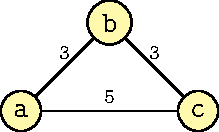
\includegraphics[width=0.6\textwidth,page=1]{distriangolare.pdf}
\end{center}
}{
Senza diseguaglianza triangolare
\begin{center}
\includegraphics[width=0.6\textwidth,page=2]{distriangolare.pdf}
\end{center}
}


\end{frame}


%-------------------------------------------------------------------------
\begin{frame}{$\Delta$-\textsc{tsp} è \NP-completo}

\BB{Dimostriamo che $\textsc{hamiltonian-circuit} \leq_p \textrm{$\Delta$-\textsc{tsp}}$}
\BIL
\item Sia $G=(V,E)$ un grafo non orientato 
\item Definiamo un insieme di distanze a partire da $G$
\medskip
\[
  d_{ij} = \begin{cases}
    1 & (i,j) \in E \\
    2 & (i,j) \notin E
  \end{cases}
\]    

\item Il grafo $G$ ha un circuito hamiltoniano se e solo se è possibile
trovare un percorso da commesso viaggiatore lungo $n$
\item Valgono le diseguaglianze triangolari: 
\medskip
\[
  d_{ij} \leq 2 \leq d_{ik}+d_{kj}
\]
\EIL
\end{frame}

%-------------------------------------------------------------------------
\begin{frame}{Lower bound per $\Delta$-\textsc{tsp}}

\BIL
\item Interpretiamo $\Delta$-\textsc{tsp} come il problema di trovare
un circuito hamiltoniano di peso minimo su un grafo completo
\item Si consideri un circuito hamiltoniano e si cancelli un suo arco
\item Si ottiene un albero di copertura
\EIL

\medskip
\IG{0.55}{toscana-hamilton.pdf}

\end{frame}

%-------------------------------------------------------------------------
\begin{frame}{Lower bound per $\Delta$-\textsc{tsp}}

\vspace{-9pt}
\begin{myboxtitle}[Teorema]
Qualunque circuito hamiltoniano $\pi$ ha costo $c(\pi)$ superiore al costo $\mathit{mst}$ di un albero di copertura di peso minimo, ovvero $\mathit{mst} < c(\pi)$
\end{myboxtitle}    

\begin{myboxtitle}[Dimostrazione]
Per assurdo
\BIL 
\item Supponiamo che esista un circuito hamiltoniano $\pi$ di costo $c(\pi) \leq \mathit{mst}$
\item Togliamo un arco, otteniamo un albero di copertura con peso inferiore
$\mathit{mst}' < c(\pi) \leq \mathit{mst}$
\item Contraddizione, visto che $\mathit{mst}$ è il costo minimo fra tutti gli alberi di copertura 
\EIL
\end{myboxtitle}

\end{frame}

%-------------------------------------------------------------------------
\begin{frame}{Algoritmo per $\Delta$-\textsc{tsp}}

\vspace{-9pt}
\BIL
\item Si individua un minimo albero di copertura di peso $\mathit{mst}$ e se ne percorrono gli archi due volte, prima in un senso e poi nell'altro 
\item In questo modo, si visita ogni città almeno una volta
\item La distanza complessiva di tale circuito è uguale a $2 \cdot \mathit{mst}$
\item Ma non è un circuito hamiltoniano!
\EIL

\vspace{-12pt}
\TwoCols{
\IG{1.0}{toscana-mst.pdf}
}{
\IG{1.0}{toscana-mst2.pdf}
}

\end{frame}

%-------------------------------------------------------------------------
\begin{frame}{Algoritmo per $\Delta$-\textsc{tsp}}

\vspace{-9pt}
\BIL
\item Si evita di passare per città già visitate - si saltano
\item Per la disuguaglianza triangolare, il costo $c(\pi)$ del circuito così
ottenuto è inferiore a $2 \cdot \mathit{mst}$
\item Quindi:
$
  c(\pi) \leq 2 \cdot \mathit{mst} < 2 \cdot c(\pi^*) \quad \Rightarrow \quad \alpha(n) < 2
$\\
dove $c(\pi^*)$ è il costo del circuito hamiltoniano ottimo
\EIL

\vspace{-12pt}
\TwoCols{
\IG{1.0}{toscana-algo.pdf}
}{
\IG{1.0}{toscana-percorso.pdf}
}

\end{frame}

%-------------------------------------------------------------------------
\begin{frame}{Algoritmo per $\Delta$-\textsc{tsp}}

\vspace{-9pt}
\begin{myboxtitle}[Note]
\BIL
\item La complessità dell'algoritmo è pari a $O(n^2 \log n)$:
  \BI
  \item $O(n^2 \log n)$ per algoritmo di Kruskal
  \item $O(n)$ per visita in profondità del MST raddoppiato con $2n$ archi
  \EI
\item Esistono grafi "perversi" per cui il fattore di approssimazione tende
al valore $2$
\item L'algoritmo di Christofides (1976) ha un fattore di approssimazione
di $3/2$, il migliore risultato al momento
\EIL
\end{myboxtitle}
  
\end{frame}

%-------------------------------------------------------------------------
\begin{frame}{Non approssimabilità di \textsc{tsp}}

\vspace{-9pt}
\begin{myboxtitle}[Teorema]
Non esiste alcun algoritmo di approssimazione assoluta per 
\textsc{tsp} tale che $c(x') \le sc(x^*)$, con $s \geq 2$ intero positivo, a meno che non sia $\PP = \NP$.
\end{myboxtitle}

\medskip
\BB{Dimostrazione}
\BIL
\item Ragionamo per assurdo; supponiamo che un tale algoritmo $A$ esista
\item Si consideri la riduzione $\textsc{hamiltonian-circuit} \leq_p \textsc{tsp}$
\item Ovvero, sia dato un grafo $G=(V,E)$ e sia $[d_{ij}]$ una
matrice di distanze tale che:
\[
d_{ij} = \begin{cases}
1, &\textrm{se $[i, j] \in E$},\\
sn, &\textrm{se $[i, j] \notin E$}.
\end{cases}
\]
\EIL

\end{frame}

%-------------------------------------------------------------------------
\begin{frame}{Non approssimabilità di \textsc{tsp}}

\vspace{-9pt}
\begin{myboxtitle}[Teorema]
Non esiste alcun algoritmo di approssimazione assoluta per il
\textsc{tsp} tale che 
\probref{Commesso viaggiatore} tale che $c(x') \le sc(x^*)$, con $s \geq 2$ intero positivo, a meno che non sia $\PP = \NP$.
\end{myboxtitle}

\medskip
\BB{Dimostrazione}
\BIL
\item Due casi:
  \BI
  \item Se $G$ ha un circuito Hamiltoniano, allora $c(x^*) = n$, quindi $A$ fornisce, in tempo polinomiale, una soluzione $x'$ tale che $c(x') \le sc(x^*) = sn$
  \item Se $G$ non ha un circuito Hamiltoniano, allora $c(x^*) > sn$, quindi
  $A$ fornisce, in tempo polinomiale, una soluzione $x'$ tale che $c(x') \geq c(x^*) > sn$
  \EI
\item Quindi $A$ risolve $\textsc{hamiltonian-circuit}$ in tempo polinomiale,
impossibile a meno che $\PP = \NP$
\EIL

\end{frame}

%%%%%%%%%%%%%%%%%%%%%%%%%%%%%%%%%%%%%%%%%%%%%%%%%%%%%%%%%%%%%%%%%%%%%%%%%%
\section{Algoritmi branch-\&-bound}

\begin{frame}{Branch-\&-bound}

\begin{myboxtitle}[Branch-\&-bound]
Per risolvere un problema di ottimizzazione NP-arduo, si può modificare la
procedura \enumerazione(), vista nella sezione su Backtrack, in modo da
"potare" certe sequenze di scelte che si rivelino incapaci di
generare la soluzione ottima
\end{myboxtitle}

\bigskip
\BB{Alcune assunzioni -- senza perdere (troppa) generalità}
\BIL
\item Problema di minimizzazione
\item Ogni sequenza di scelte abbia costo non negativo
\item Ogni scelta, aggiunta alle scelte già effettuate, non faccia 
diminuire il costo della soluzione parziale così costruita
\EIL
    
\end{frame}

\begin{frame}{Backtrack: ripasso}
    
\begin{Procedure}
\caption[A]{\BOOLEAN\ \enumerazione($\Item[\,]\ S$, \INTEGER $n$, \INTEGER\ $i$, \mldots)}
$\Set\ C = \getChoices(S, n, i, \mldots)$\REMR{Determina $C$ in funzione di $S[1 \mldots i-1]$}
\ForEach{$c \in C$}
{
  $S[i] = c$\;
  \If{$\isAdmissible(S, n, i)$}
  {
    \If{$\processSolution(S, n, i, \mldots)$}{\Return \TRUE}
  }
  \If{$\enumerazione(S, n, i+1, \mldots)$}{\Return\ \TRUE}
}
\Return \FALSE\;
\end{Procedure}
        
\end{frame}

\begin{frame}{Backtrack: ripasso}
    
\IG{1.0}{albero10.pdf}    
    
\end{frame}

\begin{frame}{Branch-\&-bound}

\BB{Upper bound per il costo della soluzione minima}
\BIL
\item Durante l'enumerazione, mantengo informazioni sulla miglior
soluzione ammissibile \Minsol e il suo costo \Mincost
\item \Mincost costituisce un \alert{limite superiore} (\alert{upper bound})
per il costo della soluzione minima
\EIL

\BB{Lower bound per il costo della soluzione minima}
\BIL
\item Si supponga di avere disposizione una opportuna funzione \alert{lower bound} $\LB(S, i)$, che:
  \BI 
  \item dipenda dalla sequenza di scelte fatte $S[1, \mldots,i]$
  \item garantisca che tutte le soluzioni ammissibili generabili facendo
nuove scelte abbiano costo $\geq \LB(S, i)$
  \EI
\EIL
    
\end{frame}

\begin{frame}{Branch-\&-bound}

\vspace{-9pt}
\begin{myboxtitle}[Potatura]
Se $\LB(S, i)$ è maggiore o uguale a \Mincost, allora si può
evitare di generare ed esplorare il sottoalbero delle scelte radicato in tal
nodo
\end{myboxtitle}

\IG{1.0}{albero10.pdf}
\end{frame}

\begin{frame}{Branch-\&-bound}

\BB{Note}
\BIL
\item Questo metodo non migliora la complessità (superpolinomiale) della procedura \enumerazione()
\item Ne abbassa drasticamente il tempo di esecuzione in pratica
\item Tutto dipende dalla funzione \LB, che deve essere il più vicino possibile al costo della soluzione ottima
\EIL

\end{frame}

\begin{frame}{Schema generale}

\vspace{-12pt}
\begin{Procedure}
\caption[A]{\branchbound($\Item[\,]\ S$, \INTEGER $n$, \INTEGER\ $i$, \mldots)}
$\Set\ C = \getChoices(S, n, i, \mldots)$\REMR{Determina $C$ in funzione di $S[1 \mldots i-1]$}
\ForEach{$c \in C$}
{
  $S[i] = c$\;
  $\INTEGER\ lb = \LB(S, i)$\;
  \If{$lb < \Mincost$}{
    \eIf{$i < n$}{
      $\branchbound(S, n, i+1, \mldots)$\;
    }{
      \If{$c(S, i) < \Mincost$}{
        $\Minsol = S$\;
        $\Mincost = c(S, i)$\;
      }
    }
  }
}
\end{Procedure}

\end{frame}

\begin{frame}{Commesso viaggiatore -- Branch-\&-bound}

\BIL
\item Sia $n$ il numero di città
\item $d[h][k]$ la distanza, intera non negativa fra le città $h$ e $k$
\item Al passo $i$-esimo sono state fatte le scelte $S[1, \mldots, i]$ 
prese dall'insieme $\{1, \mldots, n\}$
\item Un percorso ammissibile che "espande" $S[1, \mldots, i]$ deve
  \BI
  \item attraversare le città $S[1, \mldots, i]$
  \item passare da $S[i]$ ad una qualsiasi delle rimanenti $n - i$ città
  \item attraversare queste ultime città in un ordine qualsiasi
  \item da una di queste ritornare ad $S[1]$
  \EI
\EIL
\end{frame}

\begin{frame}{Commesso viaggiatore -- Branch-\&-bound}

\BIL
\item Distanza percorsa finora
\medskip
\alert{\[
C[i] = \begin{cases}
  0 & i=1 \\
  C[i-1] + d[S[i-1][S[i]] & i>1
\end{cases}
\]
}\EIL
\TwoCols{
\BIL
\item Lower bound della distanza per tornare a $S[1]$ ($O(n)$)
\medskip
\alert{\[
A = \min_{h \notin S} \{ d[h][S[1]] \}
\]
}\EIL
}{
\BIL
\item Lower bound della distanza per andarsene da $S[i]$ ($O(n)$)
\medskip
\alert{\[
B = \min_{h \notin S}\{d[S[i][\eta] \}
\]
}\EIL
}
\BIL
\item Lower bound della distanza percorsa per attraversare una
qualsiasi di queste ultime $n - i$ città, provenendo da (e dirigendosi verso)
un'altra di queste $n - i$ città ($O(n^3)$)
\medskip
\alert{\[
D[h] = \min_{p,q}\{d[p, h] + d[h, q] : h \neq p \neq q \},\;
\textrm{per ogni $h \notin S$}.
\]
}\EIL

\end{frame}

\begin{frame}{Lower bound}
Un lower bound $\LB(S)$ è dato dalla seguente espressione:

\[
\LB(s,i) = \begin{cases}
  C[i] + d[S[i], S[1]] & i=n \\
  C[i] + A + B + \left\lceil (\sum_{h \notin S} D[h])/2\right\rceil & i < n
\end{cases}
\]
\end{frame}

\begin{frame}{Commesso viaggiatore -- Branch-\&-bound}

\small
\vspace{-12pt}
\begin{Procedure}
\caption[A]{\bbTsp($\Item[\,]\ S$, $\INTARRAY\ C$, \Set $R$, \INTEGER $n$, \INTEGER\ $i$)}
\ForEach{$c \in R$}{
  $S[i] = c$\;
  $R.\setremove(c)$\;
  $C[i] = C[i - 1] + d[S[i - 1]][S[i]]$\;
  \{calcola $A$, $B$, e $D[h]$ per ogni $h \in R$\}\;
  $\INTEGER\ lb = C[i] + \IIF(i< n, \lceil ( \sum_{h \notin S} D[h]) / 2 \rceil, d[S[i]][S[1]])$\;
  \If{$lb < \Mincost$}{
    \eIf{$i < n$}{
      $\bbTsp(S, C, R, n, i+1)$\;
    }{
      $C[n] = lb$\;
      $\Minsol = S$\;
      $\Mincost = C[n]$\;
    }
  }
  $R.\setinsert(c)$\;
}
\end{Procedure}

\end{frame}

\begin{frame}{Dettagli}

\TwoColsCustom{0.55}{0.40}{
\BIL
\item $\Mincost$ è una variabile globale
\item Invece di inizializzarla a $+\infty$, possiamo scegliere una 
permutazione a caso
\item Ad esempio, la permutazione 1-2-5-3-4 ha un costo pari a 21
\item Per evitare che lo stesso circuito sia generato più volte, si
parte da un nodo fissato (es. $1$)
\EIL
}{
\includegraphics[width=\textwidth,page=9]{tsp-pentagon.pdf}
}

\end{frame}


%-------------------------------------------------------------------------
\begin{frame}{Esempio}

\IG{1.0}{branches.pdf}

\end{frame}

%-------------------------------------------------------------------------
\begin{frame}{Esempio}

\BB{
In questo semplice esempio, è stato possibile "potare" 42 su 65 nodi
}

\begin{myboxtitle}[Possibili miglioramenti]
\BIL
\item E' possibile variare l'ordine di visita dell'albero delle scelte
  \BI
  \item DFS vs Best-first
  \EI
\item E' possibile variare il meccanismo di branching
  \BI
  \item Sui nodi, sugli archi, etc.
  \EI
\item E' possibile cercare dei lower bound più stretti 
  \BI
  \item Held, M., and Karp, R. M. (1971), "The Traveling Salesman Problem and Minimum Spanning Trees: part II", Mathematical Programming 1:6-25
  \EI
\EIL
\end{myboxtitle}

\end{frame}



%%%%%%%%%%%%%%%%%%%%%%%%%%%%%%%%%%%%%%%%%%%%%%%%%%%%%%%%%%%%%%%%%%%%%%%%%%
\section{Algoritmi euristici}

%-------------------------------------------------------------------------
\begin{frame}{Algoritmi euristici}

\vspace{-9pt}
\begin{myboxtitle}[Euristiche]
Quando si è presi dalla disperazione a causa della enorme difficoltà di un
problema di ottimizzazione NP-arduo, si può ricorrere ad algoritmi
``euristici'' che forniscono una soluzione ammissibile
\BIL
\item non necessariamente ottima 
\item non necessariamente approssimata 
\EI

Dal greco antico heurískō, "Trovo, scopro”
\end{myboxtitle}

\begin{myboxtitle}[Tecniche possibili]
\BI
\item Greedy
\item Ricerca locale
\EI
\end{myboxtitle}
    
\end{frame}

%-------------------------------------------------------------------------
\begin{frame}{\textsc{tsp} -- Greedy (1)}

\vspace{-9pt}
\begin{myboxtitle}[Shortest edges first]
\BIL
\item Ordiniamo gli archi per pesi non decrescenti
\item Aggiungiamo archi alla soluzioni seguendo questo ordine finché non 
  sono stati aggiunti $n-1$ archi, dove $n$ è il numero di nodi.
\item Per poter aggiungere un arco, occorre verificare che:
  \BI
  \item per ciascuno dei suoi nodi non siano stati già scelti due archi
  \item che non si formino circuiti (\mfset)
  \EI
\item A questo punto, si è trovata una catena Hamiltoniana
\item Si chiude il circuito aggiungendo l'arco tra i due nodi estremi della catena
\EIL
\end{myboxtitle}

\end{frame}


%-------------------------------------------------------------------------
\begin{frame}{Esempio}

\TwoCols{
\vspace{-18pt}
\IG{1.0}{tsp-greedy.pdf}
}{
\includegraphics<1|handout:1>[width=\textwidth,page=1]{tsp-pentagon.pdf}
\includegraphics<2|handout:0>[width=\textwidth,page=2]{tsp-pentagon.pdf}
\includegraphics<3|handout:0>[width=\textwidth,page=3]{tsp-pentagon.pdf}
\includegraphics<4|handout:0>[width=\textwidth,page=4]{tsp-pentagon.pdf}
\includegraphics<5|handout:0>[width=\textwidth,page=5]{tsp-pentagon.pdf}
\includegraphics<6|handout:0>[width=\textwidth,page=6]{tsp-pentagon.pdf}
\includegraphics<7|handout:0>[width=\textwidth,page=7]{tsp-pentagon.pdf}
\includegraphics<8|handout:2>[width=\textwidth,page=8]{tsp-pentagon.pdf}
}

\alert{
\bigskip
\onslide<8|handout:2>Costo: $21$
}


\end{frame}

%-------------------------------------------------------------------------
\begin{frame}[shrink=10]{\textsc{tsp} -- Greedy (1)}

\vspace{-12pt}
\begin{Procedure}
\caption[A]{\Set\ \greedyTsp(\Graph $G$)}
$\Set\ S = \setconstructor()$\;
$\mfset\ M = \mfconstructor(G.n)$\;
$\INTEGER[\,]\ \Inc = \NEW\ \INTEGER[1 \ldots n]$\;
\lFor{$i = 1$ \TO\ $G.n$}{$\Inc[i] = 0$}
\{ ordina gli archi per peso non decrescente \}\;
\ForEach{$[u,v] \in G.E$}{
  \If{$\Inc[u] < 2$ \AND $\Inc[v]<2$ \AND $M.\mffind(u) \neq M.\mffind(v)$}{
    $S.\setinsert([u,v])$\;
    $\Inc[u] = \Inc[u]+1$\;
    $\Inc[v] = \Inc[v]+1$\;
    $M.\mfmerge(u,v)$\;
  }
}
\INTEGER $u = 1$;
\lWhile{$\Inc[u] \neq 1$}{$u = u+1$}
\INTEGER $v = u+1$; 
\lWhile{$\Inc[v] \neq 1$}{$v = v+1$}
$S.\setinsert([u,v])$\;
\Return $S$\;
\end{Procedure}

\end{frame}



%-------------------------------------------------------------------------
\begin{frame}{\textsc{tsp} -- Greedy (2)}

\vspace{-9pt}
\begin{myboxtitle}[Nearest neighbor]
\BIL
\item Si parte da una città
\item Si seleziona come prossima città quella più vicina
\item Si va avanti così, evitando città già visitate
\item Quando si sono visitate tutte le città, si torna alla città di
partenza
\item Si può lavorare direttamente sulla matrice
\EIL
\end{myboxtitle}

\end{frame}

%-------------------------------------------------------------------------
\begin{frame}{\textsc{tsp} -- Greedy (2)}

\TwoCols{
\vspace{-18pt}
\IG{1.0}{tsp-greedy.pdf}
}{
\includegraphics<1|handout:1>[width=\textwidth,page=1]{tsp-nn.pdf}
\includegraphics<2|handout:0>[width=\textwidth,page=2]{tsp-nn.pdf}
\includegraphics<3|handout:0>[width=\textwidth,page=3]{tsp-nn.pdf}
\includegraphics<4|handout:0>[width=\textwidth,page=4]{tsp-nn.pdf}
\includegraphics<5|handout:0>[width=\textwidth,page=5]{tsp-nn.pdf}
\includegraphics<6|handout:2>[width=\textwidth,page=6]{tsp-nn.pdf}
}

\alert{
\bigskip
\onslide<6|handout:2>Costo: $21$
}


\end{frame}


%-------------------------------------------------------------------------
\begin{frame}{\textsc{tsp} -- Greedy}

\BIL
\item Costo computazionale:
  \BI
  \item Greedy 1: $O(n^2 \log n)$ (ordinamento archi)
  \item Greedy 2: $O(n^2)$
  \EI
\item La soluzione così ottenuta si può utilizzare come:
\BI
\item base di partenza per un algoritmo branch-\&-bound
\item può essere migliorata ancora tramite ricerca locale
\EI
\EIL

\end{frame}


%-------------------------------------------------------------------------
\begin{frame}{\textsc{tsp} -- Approccio ricerca locale}

\vspace{-9pt}
\begin{myboxtitle}[Ricerca locale]
Sia $\pi$ un circuito Hamiltoniano del grafo completo derivante dal problema
\textsc{tsp}. Si consideri il seguente intorno:
\[
I_2(\pi) = \parbox[t]{9cm}{\{$\pi'$: $\pi'$ è ottenuto da
$\pi$ cancellando due archi non consecutivi del circuito e
sostituendoli con due archi esterni al circuito\}}
\]
\end{myboxtitle}

\begin{myboxtitle}[Note]
\BIL
\item $|I_2(\pi)| = n(n - 1)/2 - n$
  \BI
  \item Ci sono $n(n-1)/2$ coppie di archi del circuito
  \item $n$ di esse sono consecutive
  \item Una volta spezzato un circuito, esiste un solo modo per riconnetterlo
  \EI
\item Costo per esaminare $I_2(\pi)$: $O(n^2)$
\EIL
\end{myboxtitle}

\end{frame}

%-------------------------------------------------------------------------
\begin{frame}{Esempio}

\TwoCols{
\vspace{-18pt}
\IG{1.0}{tsp-greedy.pdf}
}{
\includegraphics<1|handout:1>[width=\textwidth,page=1]{tsp-local.pdf}
\includegraphics<2|handout:0>[width=\textwidth,page=2]{tsp-local.pdf}
\includegraphics<3|handout:2>[width=\textwidth,page=3]{tsp-local.pdf}
\includegraphics<4|handout:0>[width=\textwidth,page=4]{tsp-local.pdf}
\includegraphics<5|handout:3>[width=\textwidth,page=5]{tsp-local.pdf}
}

\alert{
\bigskip
\begin{overprint}
\onslide<1-2|handout:1>Costo: $25$
\onslide<3-4|handout:2>Costo: $23$
\onslide<5|handout:3>Costo: $19$
\end{overprint}
}

\end{frame}

%-------------------------------------------------------------------------
\begin{frame}{Spunti di lettura}

\begin{myboxtitle}[Bibliografia]
\BIL
\item Rego, César; Gamboa, Dorabela; Glover, Fred; Osterman, Colin (2011), "Traveling salesman problem heuristics: leading methods, implementations and latest advances", European Journal of Operational Research, 211 (3): 427–441.
\url{https://www.sciencedirect.com/science/article/pii/S0377221710006065?via\%3Dihub}

\item David Williamson, David Shmoys (2010). The Design of Approximation Algorithms. Cambridge University Press.\\
\url{http://www.designofapproxalgs.com/book.pdf}

\item David Williamson, David Shmoys (2010). The Design of Approximation Algorithms. Cambridge University Press.\\
\url{http://www.designofapproxalgs.com/book.pdf}
\EIL
\end{myboxtitle}


\end{frame}


%%%%%%%%%%%%%%%%%%%%%%%%%%%%%%%%%%%%%%%%%%%%%%%%%%%%%%%%%%%%%%%%%%%%%%%%%%
\end{document}






%-------------------------------------------------------------------------
\begin{frame}{}

\end{frame}




